\chapter{Weighted scatterplots}

In this chapter, we will work towards creating the weighted scatterplot
below. We will take you from a basic scatterplot and explain all the
customisations we add to the code step-by-step.

\begin{center}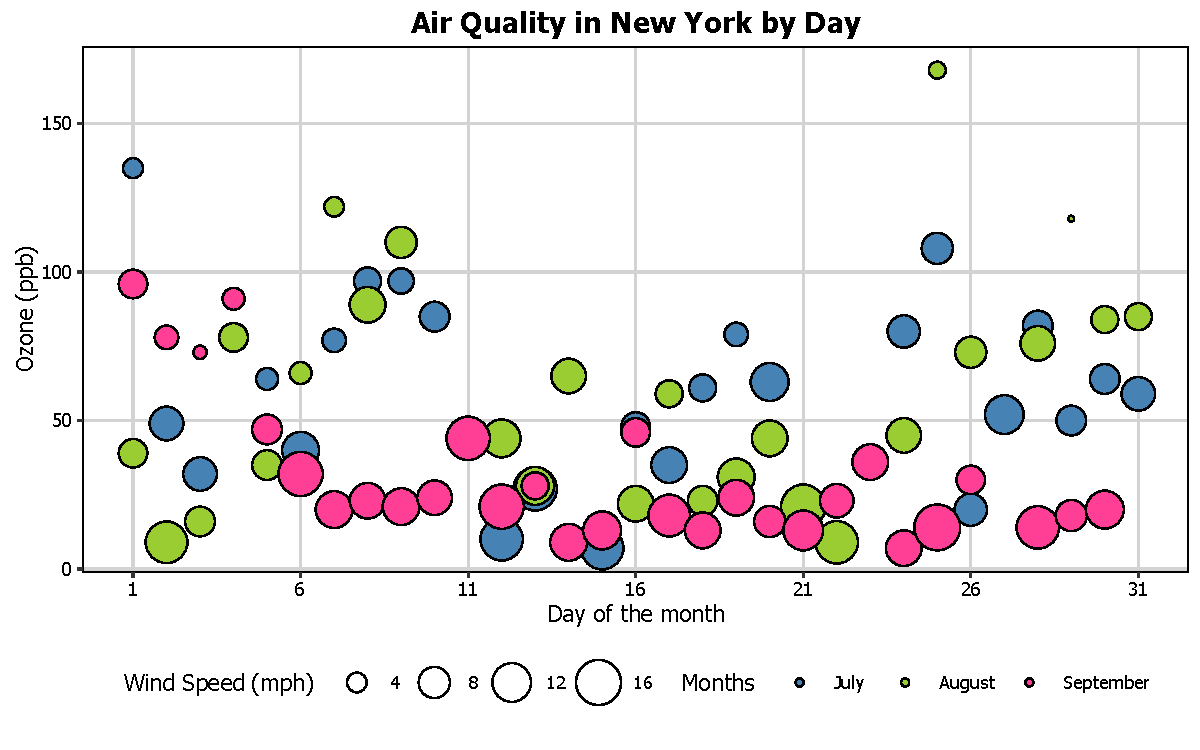
\includegraphics[width=0.6\linewidth]{6_Weighted_Scatterplots_pdf/wscatter_finalgraph-1} \end{center}

The first thing to do is load in the data, as below:

\begin{Shaded}
\begin{Highlighting}[]
\KeywordTok{library}\NormalTok{(ggplot2)}
\KeywordTok{library}\NormalTok{(ggthemes)}
\KeywordTok{library}\NormalTok{(extrafont)}
\KeywordTok{library}\NormalTok{(plyr)}
\KeywordTok{library}\NormalTok{(scales)}

\KeywordTok{data}\NormalTok{(airquality)}
\end{Highlighting}
\end{Shaded}

We will then trim the data down to the final three months and turn the
\texttt{Month} variable into a labelled factor variable. We end up with
a new dataset called \texttt{aq\_trim}.

\begin{Shaded}
\begin{Highlighting}[]
\NormalTok{aq_trim <-}\StringTok{ }\NormalTok{airquality[}\KeywordTok{which}\NormalTok{(airquality$Month ==}\StringTok{ }\DecValTok{7} \NormalTok{|}
\NormalTok{airquality$Month ==}\StringTok{ }\DecValTok{8} \NormalTok{|}
\NormalTok{airquality$Month ==}\StringTok{ }\DecValTok{9}\NormalTok{), ]}
\NormalTok{aq_trim$Month <-}\StringTok{ }\KeywordTok{factor}\NormalTok{(aq_trim$Month, }
\DataTypeTok{labels =} \KeywordTok{c}\NormalTok{(}\StringTok{"July"}\NormalTok{, }\StringTok{"August"}\NormalTok{, }\StringTok{"September"}\NormalTok{))}
\end{Highlighting}
\end{Shaded}

\section{Basic weighted scatterplot}\label{basic-weighted-scatterplot}

Let's start really slowly by revisiting how to create a basic
scatterplot. In order to initialise this plot we tell ggplot that
\texttt{aq\_trim} is our data, and specify that our x-axis plots the
\texttt{Day} variable and our y-axis plots the \texttt{Ozone} variable.
We then instruct ggplot to render this as a scatterplot by adding the
\texttt{geom\_point()} option.

\begin{Shaded}
\begin{Highlighting}[]
\NormalTok{p6 <-}\StringTok{ }\KeywordTok{ggplot}\NormalTok{(aq_trim, }\KeywordTok{aes}\NormalTok{(}\DataTypeTok{x =} \NormalTok{Day, }\DataTypeTok{y =} \NormalTok{Ozone)) +}\StringTok{ }
\StringTok{      }\KeywordTok{geom_point}\NormalTok{()}
\NormalTok{p6}
\end{Highlighting}
\end{Shaded}

\begin{center}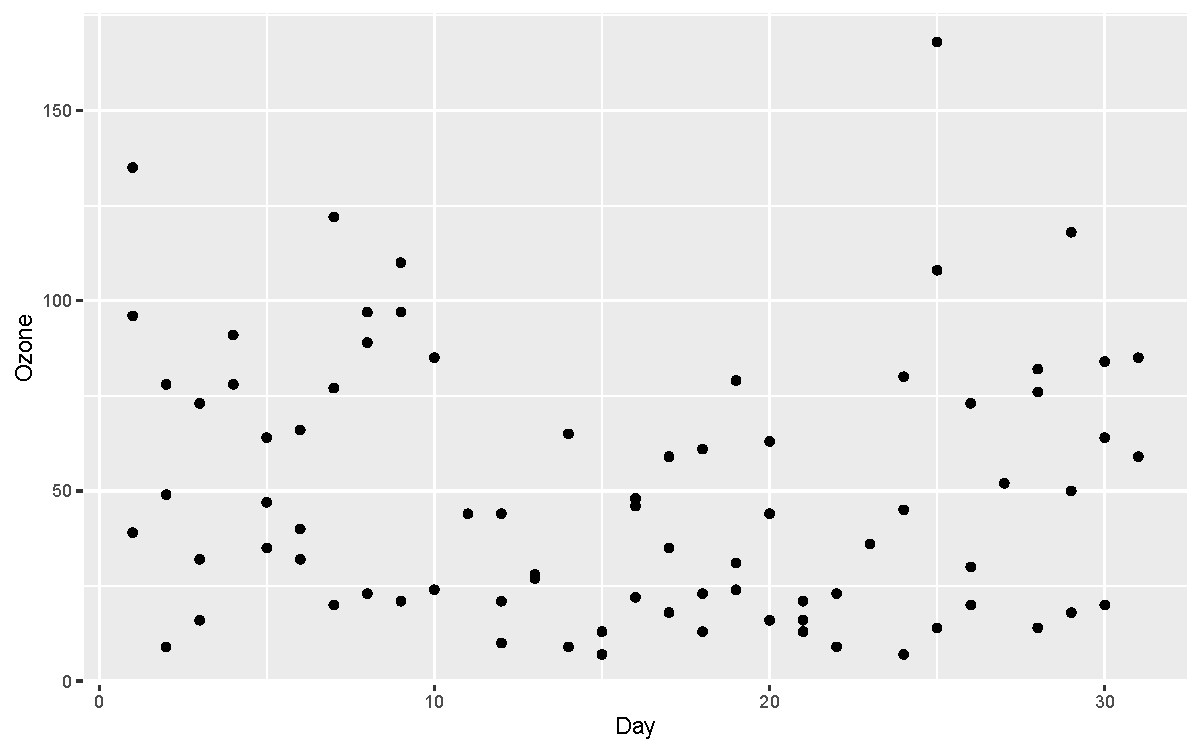
\includegraphics[width=0.6\linewidth]{6_Weighted_Scatterplots_pdf/wscatter_1-1} \end{center}

In order to turn this into a weighted scatterplot, we simply add the
\texttt{size} argument to \texttt{ggplot(aes())}. In this case, we want
to weight the points by the \texttt{Wind} variable.

\begin{Shaded}
\begin{Highlighting}[]
\NormalTok{p6 <-}\StringTok{ }\KeywordTok{ggplot}\NormalTok{(aq_trim, }\KeywordTok{aes}\NormalTok{(}\DataTypeTok{x =} \NormalTok{Day, }\DataTypeTok{y =} \NormalTok{Ozone, }\DataTypeTok{size =} \NormalTok{Wind)) +}\StringTok{ }
\StringTok{  }\KeywordTok{geom_point}\NormalTok{()}
\NormalTok{p6}
\end{Highlighting}
\end{Shaded}

\begin{center}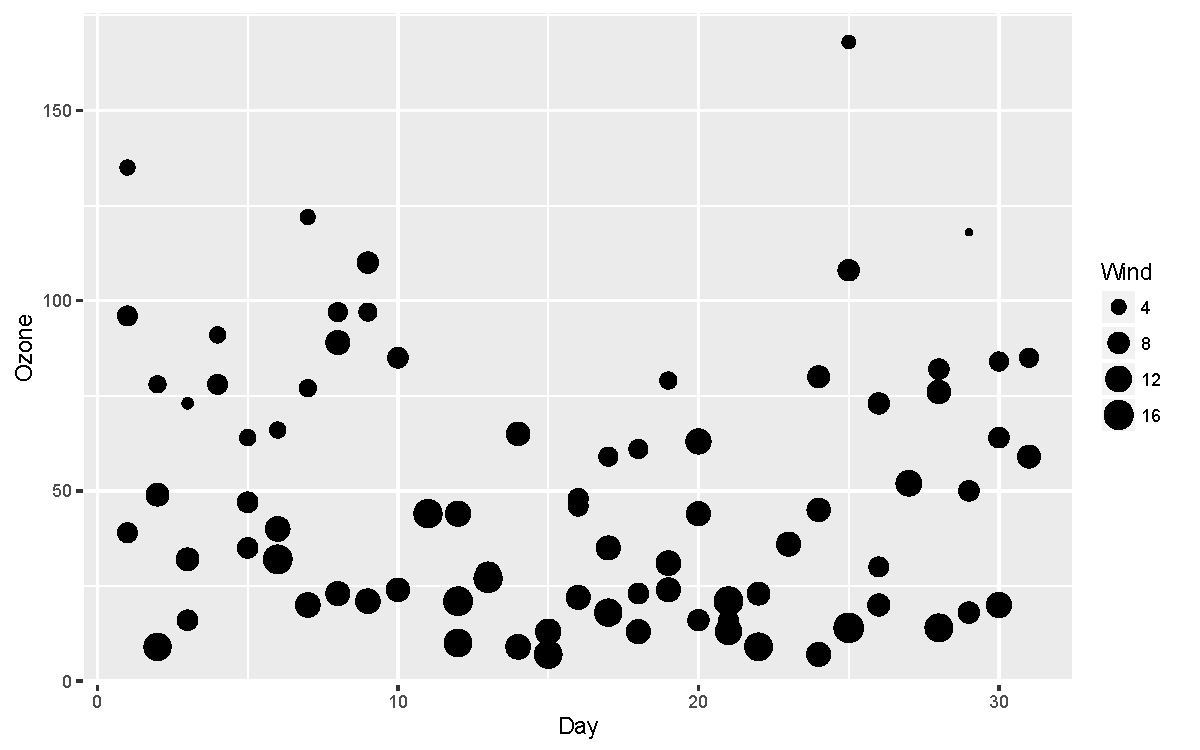
\includegraphics[width=0.6\linewidth]{6_Weighted_Scatterplots_pdf/wscatter_2-1} \end{center}

You can see we already have an interesting looking pattern, where days
with higher wind speed tend to have lower ozone (or in other words,
better air quality). Now let's make it beautiful!

\section{Changing the shape of the data
points}\label{changing-the-shape-of-the-data-points}

Perhaps we want the data points to be a different shape than a solid
circle. We can change these by adding the \texttt{shape} argument to
\texttt{geom\_point}. An explanation of the allowed arguments for shape
are described in
\href{http://sape.inf.usi.ch/quick-reference/ggplot2/shape}{this
article}. In this case, we will use shape 21, which is a circle that
allows different colours for the outline and fill.

\begin{Shaded}
\begin{Highlighting}[]
\NormalTok{p6 <-}\StringTok{ }\KeywordTok{ggplot}\NormalTok{(aq_trim, }\KeywordTok{aes}\NormalTok{(}\DataTypeTok{x =} \NormalTok{Day, }\DataTypeTok{y =} \NormalTok{Ozone, }\DataTypeTok{size =} \NormalTok{Wind)) +}\StringTok{ }
\StringTok{  }\KeywordTok{geom_point}\NormalTok{(}\DataTypeTok{shape =} \DecValTok{21}\NormalTok{)}
\NormalTok{p6}
\end{Highlighting}
\end{Shaded}

\begin{center}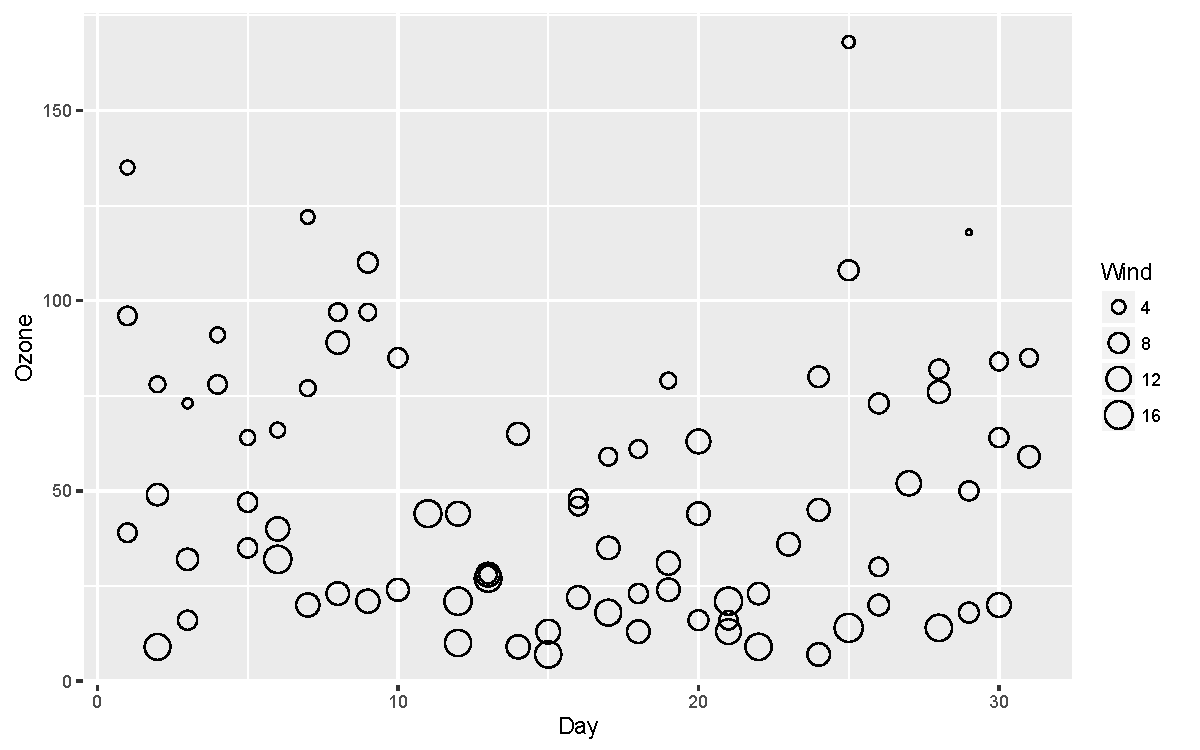
\includegraphics[width=0.6\linewidth]{6_Weighted_Scatterplots_pdf/wscatter_3-1} \end{center}

\section{Adjusting the axis scales}\label{adjusting-the-axis-scales}

To change the x-axis tick marks, we use the
\texttt{scale\_x\_continuous} option. Similarly, to change the y-axis we
use the \texttt{scale\_y\_continuous} option. Here we will change the
x-axis to every 5 days, rather than 10, and change the range from 1 to
31 (as 0 is not a valid value for this variable).

\begin{Shaded}
\begin{Highlighting}[]
\NormalTok{p6 <-}\StringTok{ }\NormalTok{p6 +}\StringTok{ }\KeywordTok{scale_x_continuous}\NormalTok{(}\DataTypeTok{breaks =} \KeywordTok{seq}\NormalTok{(}\DecValTok{1}\NormalTok{, }\DecValTok{31}\NormalTok{, }\DecValTok{5}\NormalTok{))}
\NormalTok{p6}
\end{Highlighting}
\end{Shaded}

\begin{center}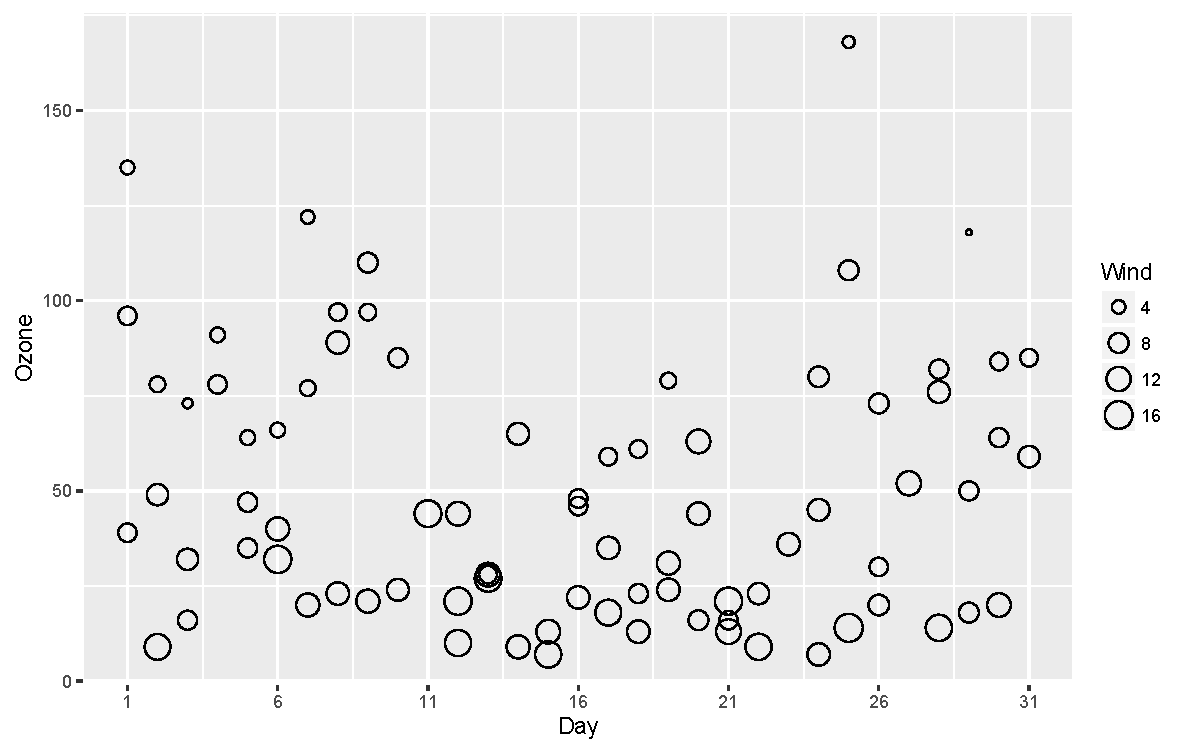
\includegraphics[width=0.6\linewidth]{6_Weighted_Scatterplots_pdf/wscatter_4-1} \end{center}

\section{Adjusting axis labels \& adding
title}\label{adjusting-axis-labels-adding-title}

To add a title, we include the option \texttt{ggtitle} and include the
name of the graph as a string argument. To change the axis names we add
\texttt{x} and \texttt{y} arguments to the \texttt{labs} command.

\begin{Shaded}
\begin{Highlighting}[]
\NormalTok{p6 <-}\StringTok{ }\NormalTok{p6 +}\StringTok{ }\KeywordTok{ggtitle}\NormalTok{(}\StringTok{"Air Quality in New York by Day"}\NormalTok{) +}\StringTok{ }
\StringTok{  }\KeywordTok{labs}\NormalTok{(}\DataTypeTok{x =} \StringTok{"Day of the month"}\NormalTok{, }\DataTypeTok{y =} \StringTok{"Ozone (ppb)"}\NormalTok{) }
\NormalTok{p6}
\end{Highlighting}
\end{Shaded}

\begin{center}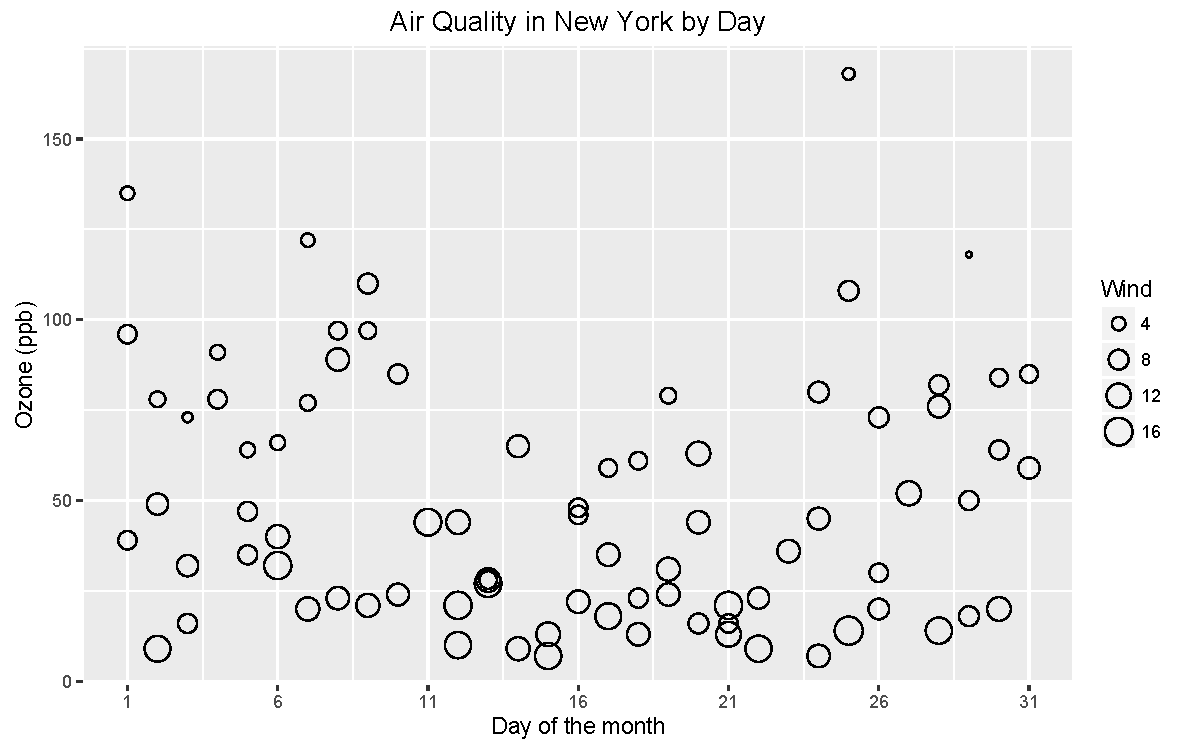
\includegraphics[width=0.6\linewidth]{6_Weighted_Scatterplots_pdf/wscatter_5-1} \end{center}

\section{Adjusting the colour
palette}\label{adjusting-the-colour-palette}

There are a few options for adjusting the colour. The most simple is to
make every point one fixed colour. You can reference colours by name,
with the full list of colours recognised by R
\href{http://www.stat.columbia.edu/~tzheng/files/Rcolor.pdf}{here}.
Let's try making the outline \texttt{mediumvioletred} and the fill
\texttt{springgreen}.

\begin{Shaded}
\begin{Highlighting}[]
\NormalTok{p6 <-}\StringTok{ }\KeywordTok{ggplot}\NormalTok{(aq_trim, }\KeywordTok{aes}\NormalTok{(}\DataTypeTok{x =} \NormalTok{Day, }\DataTypeTok{y =} \NormalTok{Ozone, }\DataTypeTok{size =} \NormalTok{Wind)) +}\StringTok{ }
\StringTok{  }\KeywordTok{geom_point}\NormalTok{(}\DataTypeTok{shape =} \DecValTok{21}\NormalTok{, }\DataTypeTok{colour =} \StringTok{"mediumvioletred"}\NormalTok{, }\DataTypeTok{fill =} \StringTok{"springgreen"}\NormalTok{) +}
\StringTok{  }\KeywordTok{ggtitle}\NormalTok{(}\StringTok{"Air Quality in New York by Day"}\NormalTok{) +}\StringTok{ }
\StringTok{  }\KeywordTok{labs}\NormalTok{(}\DataTypeTok{x =} \StringTok{"Day of the month"}\NormalTok{, }\DataTypeTok{y =} \StringTok{"Ozone (ppb)"}\NormalTok{) +}
\StringTok{  }\KeywordTok{scale_x_continuous}\NormalTok{(}\DataTypeTok{breaks =} \KeywordTok{seq}\NormalTok{(}\DecValTok{1}\NormalTok{, }\DecValTok{31}\NormalTok{, }\DecValTok{5}\NormalTok{)) }
\NormalTok{p6}
\end{Highlighting}
\end{Shaded}

\begin{center}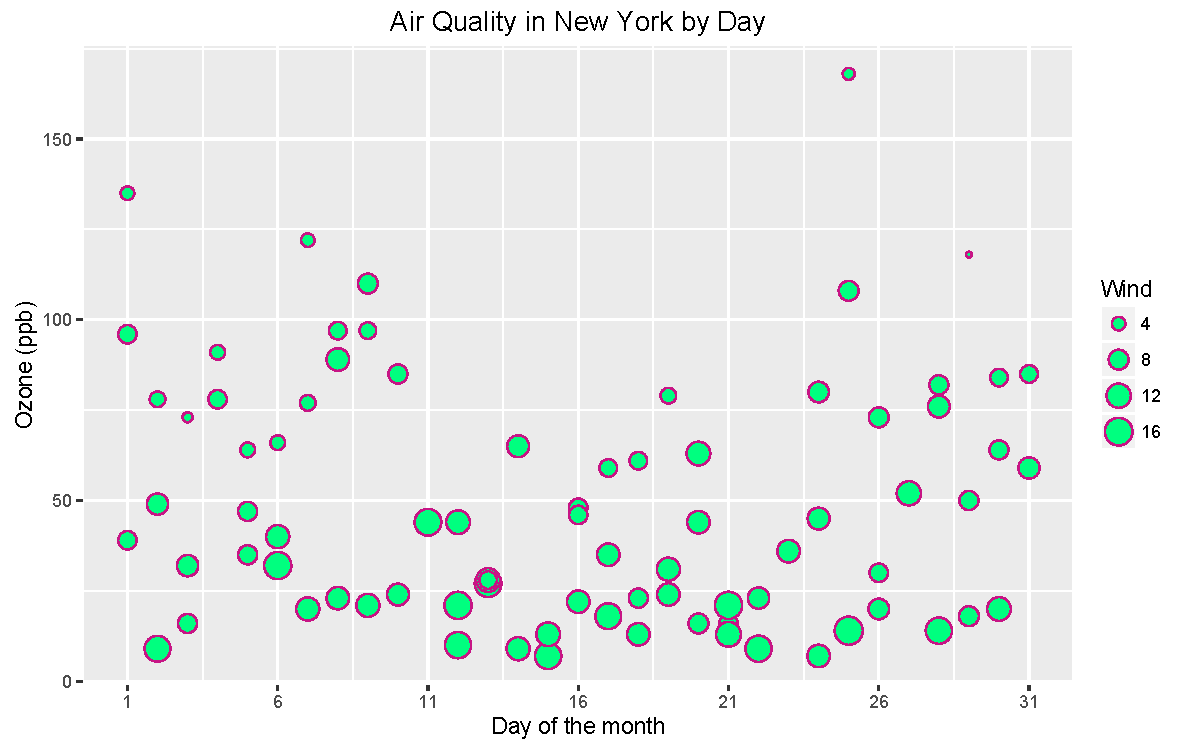
\includegraphics[width=0.6\linewidth]{6_Weighted_Scatterplots_pdf/wscatter_6-1} \end{center}

You can change the colours using specific HEX codes instead. Here we
have made the outline \#000000 (black) and the fill ``\#40b8d0 (vivid
cyan).

\begin{Shaded}
\begin{Highlighting}[]
\NormalTok{p6 <-}\StringTok{ }\KeywordTok{ggplot}\NormalTok{(aq_trim, }\KeywordTok{aes}\NormalTok{(}\DataTypeTok{x =} \NormalTok{Day, }\DataTypeTok{y =} \NormalTok{Ozone, }\DataTypeTok{size =} \NormalTok{Wind)) +}\StringTok{ }
\StringTok{  }\KeywordTok{geom_point}\NormalTok{(}\DataTypeTok{shape =} \DecValTok{21}\NormalTok{, }\DataTypeTok{colour =} \StringTok{"#000000"}\NormalTok{, }\DataTypeTok{fill =} \StringTok{"#40b8d0"}\NormalTok{) +}
\StringTok{  }\KeywordTok{ggtitle}\NormalTok{(}\StringTok{"Air Quality in New York by Day"}\NormalTok{) +}\StringTok{ }
\StringTok{  }\KeywordTok{labs}\NormalTok{(}\DataTypeTok{x =} \StringTok{"Day of the month"}\NormalTok{, }\DataTypeTok{y =} \StringTok{"Ozone (ppb)"}\NormalTok{) +}
\StringTok{  }\KeywordTok{scale_x_continuous}\NormalTok{(}\DataTypeTok{breaks =} \KeywordTok{seq}\NormalTok{(}\DecValTok{1}\NormalTok{, }\DecValTok{31}\NormalTok{, }\DecValTok{5}\NormalTok{))}
\NormalTok{p6}
\end{Highlighting}
\end{Shaded}

\begin{center}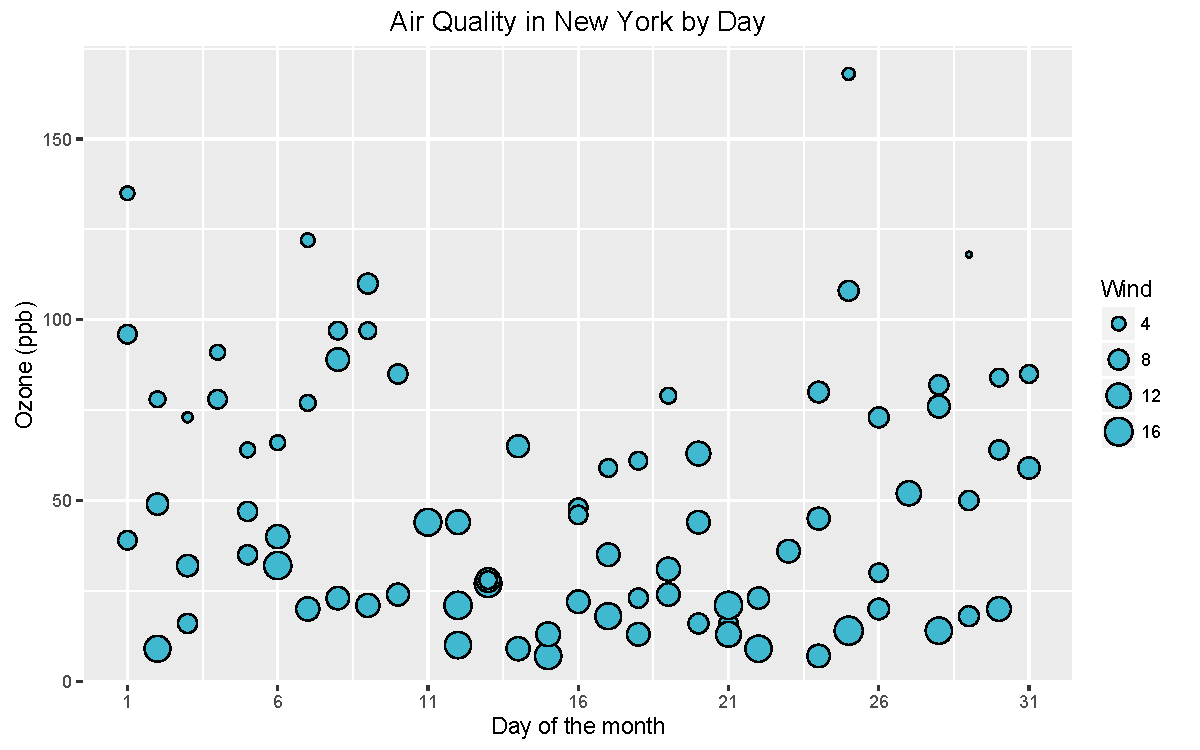
\includegraphics[width=0.6\linewidth]{6_Weighted_Scatterplots_pdf/wscatter_7-1} \end{center}

You can also change the colour of the data points according to the
levels of another variable. This can be done either as a continuous
gradient, or as a levels of a factor variable. Let's change the colour
by the values of temperature:

\begin{Shaded}
\begin{Highlighting}[]
\NormalTok{p6 <-}\StringTok{ }\KeywordTok{ggplot}\NormalTok{(aq_trim, }\KeywordTok{aes}\NormalTok{(}\DataTypeTok{x =} \NormalTok{Day, }\DataTypeTok{y =} \NormalTok{Ozone, }\DataTypeTok{size =} \NormalTok{Wind, }\DataTypeTok{fill =} \NormalTok{Temp)) +}\StringTok{ }
\StringTok{  }\KeywordTok{geom_point}\NormalTok{(}\DataTypeTok{shape =} \DecValTok{21}\NormalTok{) +}
\StringTok{  }\KeywordTok{ggtitle}\NormalTok{(}\StringTok{"Air Quality in New York by Day"}\NormalTok{) +}\StringTok{ }
\StringTok{  }\KeywordTok{labs}\NormalTok{(}\DataTypeTok{x =} \StringTok{"Day of the month"}\NormalTok{, }\DataTypeTok{y =} \StringTok{"Ozone (ppb)"}\NormalTok{) +}
\StringTok{  }\KeywordTok{scale_x_continuous}\NormalTok{(}\DataTypeTok{breaks =} \KeywordTok{seq}\NormalTok{(}\DecValTok{1}\NormalTok{, }\DecValTok{31}\NormalTok{, }\DecValTok{5}\NormalTok{))}
\NormalTok{p6}
\end{Highlighting}
\end{Shaded}

\begin{center}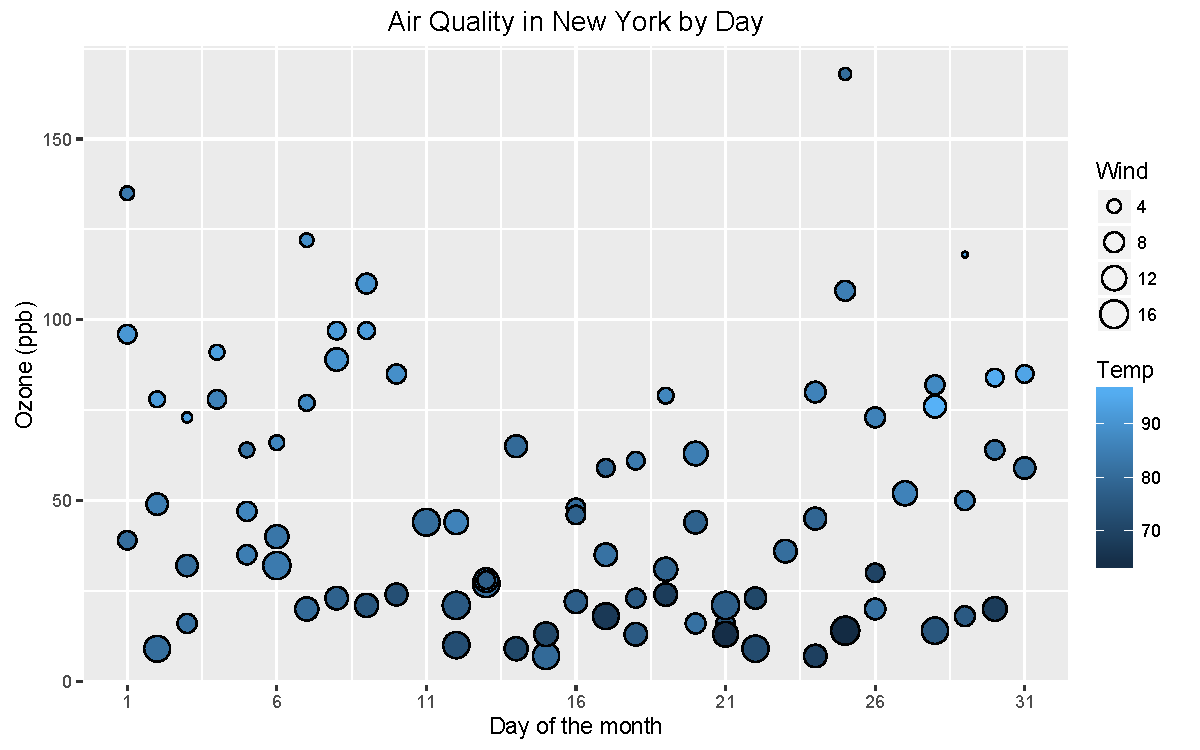
\includegraphics[width=0.6\linewidth]{6_Weighted_Scatterplots_pdf/wscatter_8-1} \end{center}

We can change the gradient's colours by adding the
\texttt{scale\_fill\_continuous} option. The \texttt{low} and
\texttt{high} arguments specify the range of colours the gradient should
transition between.

\begin{Shaded}
\begin{Highlighting}[]
\NormalTok{p6 <-p6 +}\StringTok{ }\KeywordTok{scale_fill_continuous}\NormalTok{(}\DataTypeTok{low =} \StringTok{"plum1"}\NormalTok{, }\DataTypeTok{high =} \StringTok{"purple4"}\NormalTok{)}
\NormalTok{p6}
\end{Highlighting}
\end{Shaded}

\begin{center}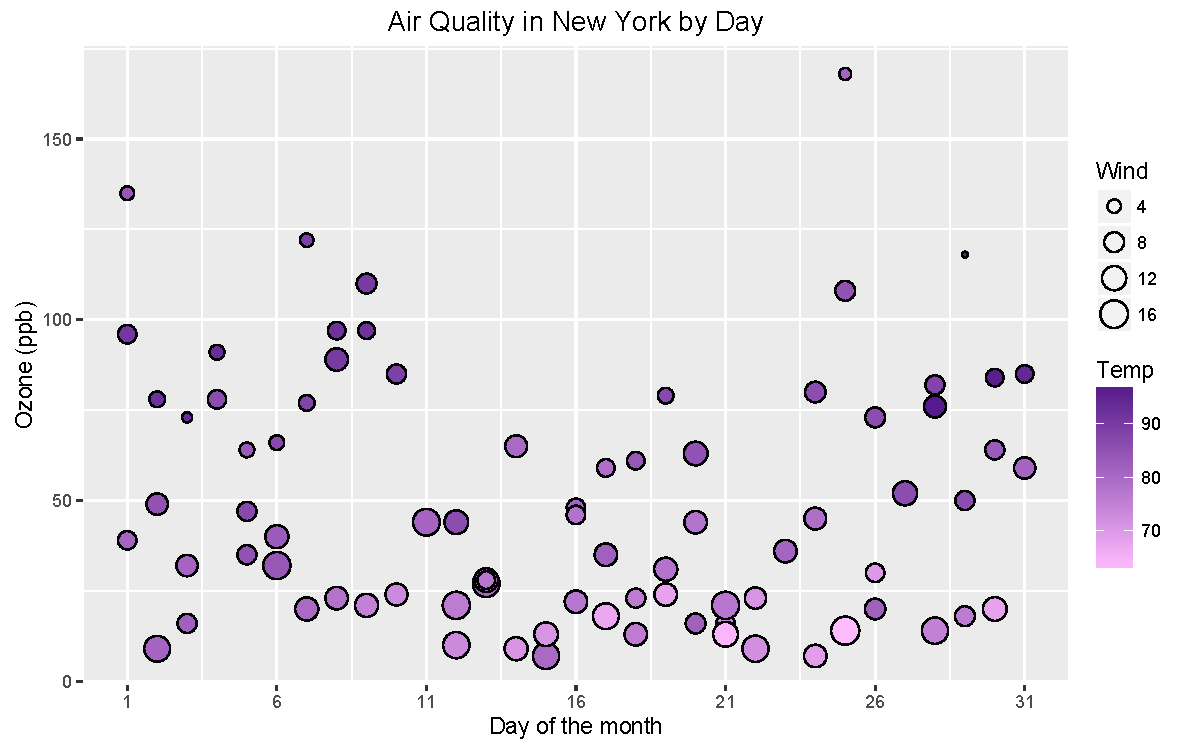
\includegraphics[width=0.6\linewidth]{6_Weighted_Scatterplots_pdf/wscatter_9-1} \end{center}

We can see that higher temperatures seem to have higher ozone levels.

Let's now change the colours of the data points by a factor variable,
\texttt{Month}.

\begin{Shaded}
\begin{Highlighting}[]
\NormalTok{p6 <-}\StringTok{ }\KeywordTok{ggplot}\NormalTok{(aq_trim, }\KeywordTok{aes}\NormalTok{(}\DataTypeTok{x =} \NormalTok{Day, }\DataTypeTok{y =} \NormalTok{Ozone, }\DataTypeTok{size =} \NormalTok{Wind, }\DataTypeTok{fill =} \NormalTok{Month)) +}\StringTok{ }
\StringTok{  }\KeywordTok{geom_point}\NormalTok{(}\DataTypeTok{shape =} \DecValTok{21}\NormalTok{) +}
\StringTok{  }\KeywordTok{ggtitle}\NormalTok{(}\StringTok{"Air Quality in New York by Day"}\NormalTok{) +}\StringTok{ }
\StringTok{  }\KeywordTok{labs}\NormalTok{(}\DataTypeTok{x =} \StringTok{"Day of the month"}\NormalTok{, }\DataTypeTok{y =} \StringTok{"Ozone (ppb)"}\NormalTok{) +}
\StringTok{  }\KeywordTok{scale_x_continuous}\NormalTok{(}\DataTypeTok{breaks =} \KeywordTok{seq}\NormalTok{(}\DecValTok{1}\NormalTok{, }\DecValTok{31}\NormalTok{, }\DecValTok{5}\NormalTok{))}
\NormalTok{p6}
\end{Highlighting}
\end{Shaded}

\begin{center}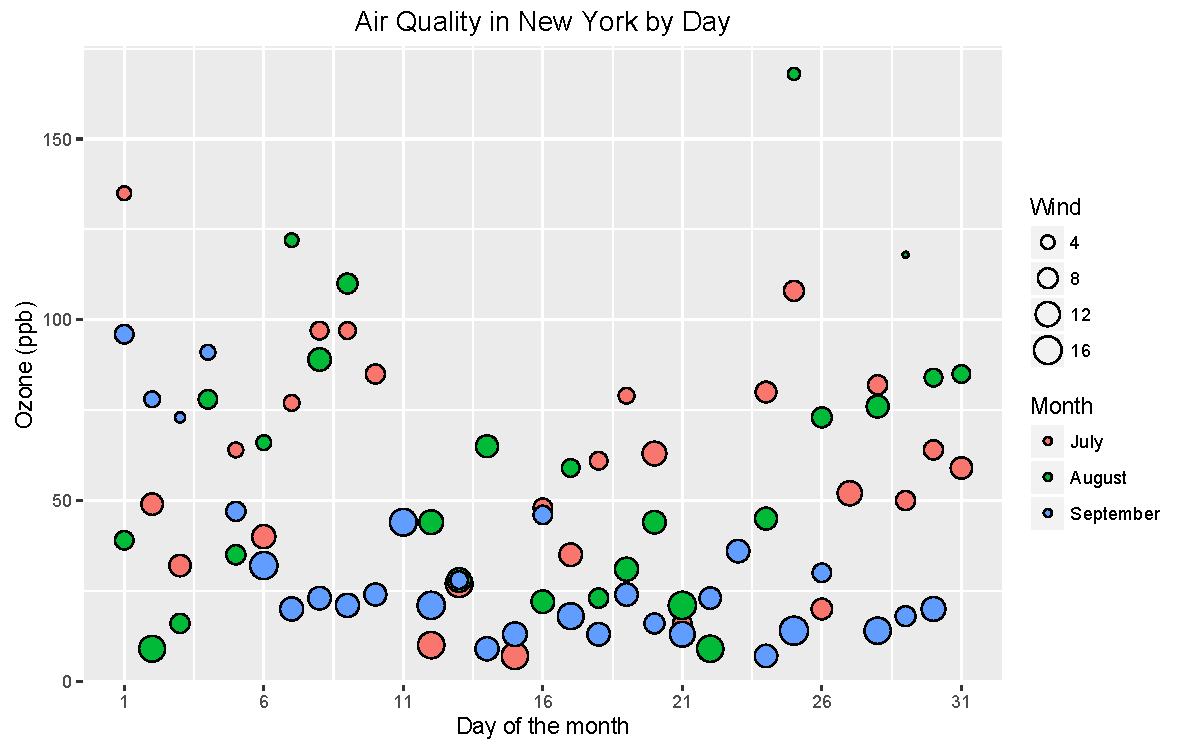
\includegraphics[width=0.6\linewidth]{6_Weighted_Scatterplots_pdf/wscatter_10-1} \end{center}

Again, we can change the colours of these data points, this time using
\texttt{scale\_fill\_manual}.

\begin{Shaded}
\begin{Highlighting}[]
\NormalTok{fill =}\StringTok{ }\KeywordTok{c}\NormalTok{(}\StringTok{"steelblue"}\NormalTok{, }\StringTok{"yellowgreen"}\NormalTok{, }\StringTok{"violetred1"}\NormalTok{)}

\NormalTok{p6 <-}\StringTok{ }\NormalTok{p6 +}\StringTok{ }\KeywordTok{scale_fill_manual}\NormalTok{(}\DataTypeTok{values =} \NormalTok{fill)}
\NormalTok{p6}
\end{Highlighting}
\end{Shaded}

\begin{center}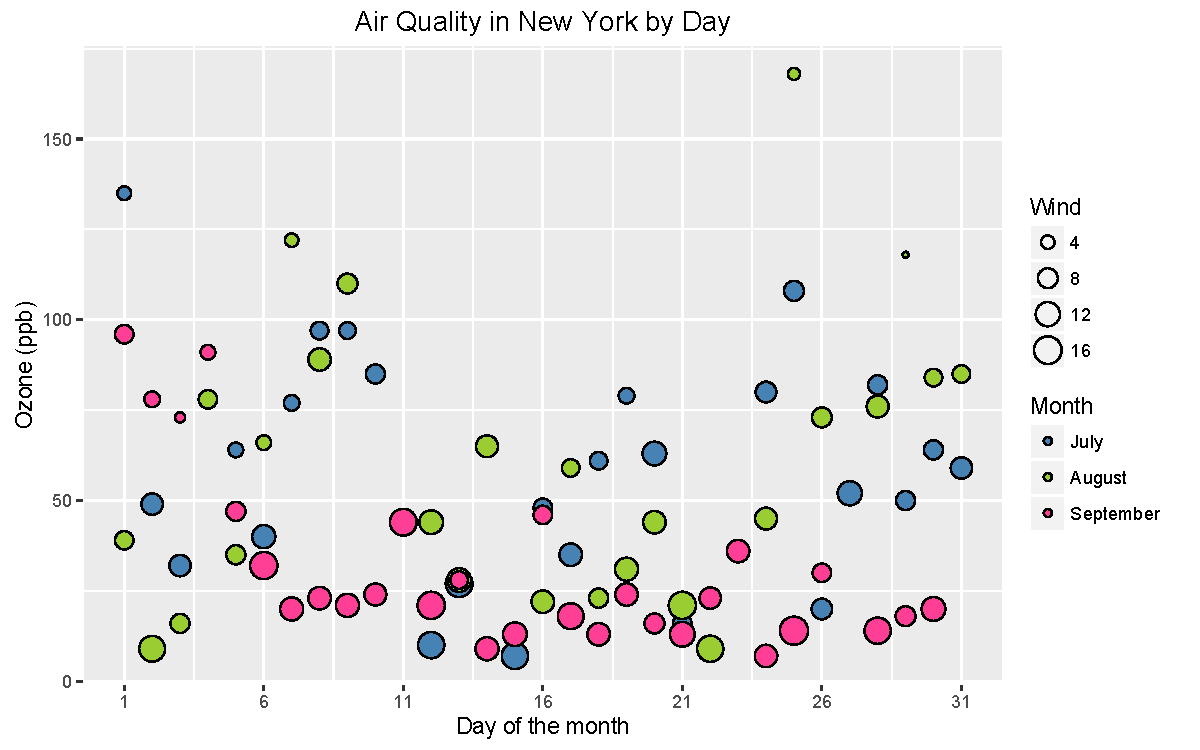
\includegraphics[width=0.6\linewidth]{6_Weighted_Scatterplots_pdf/wscatter_11-1} \end{center}

\section{Adjusting the size of the data
points}\label{adjusting-the-size-of-the-data-points}

The default size of the the data points in a weighted scatterplot is
mapped to the radius of the plots. If we want the data points to be
proportional to the value of the weighting variable (e.g., a wind speed
of 0 mph would have a value of 0), we need to use the
\texttt{scale\_size\_area}.

\begin{Shaded}
\begin{Highlighting}[]
\NormalTok{p6 <-}\StringTok{ }\NormalTok{p6 +}\StringTok{ }\KeywordTok{scale_size_area}\NormalTok{(}\DataTypeTok{max_size =} \DecValTok{10}\NormalTok{)}
\NormalTok{p6}
\end{Highlighting}
\end{Shaded}

\begin{center}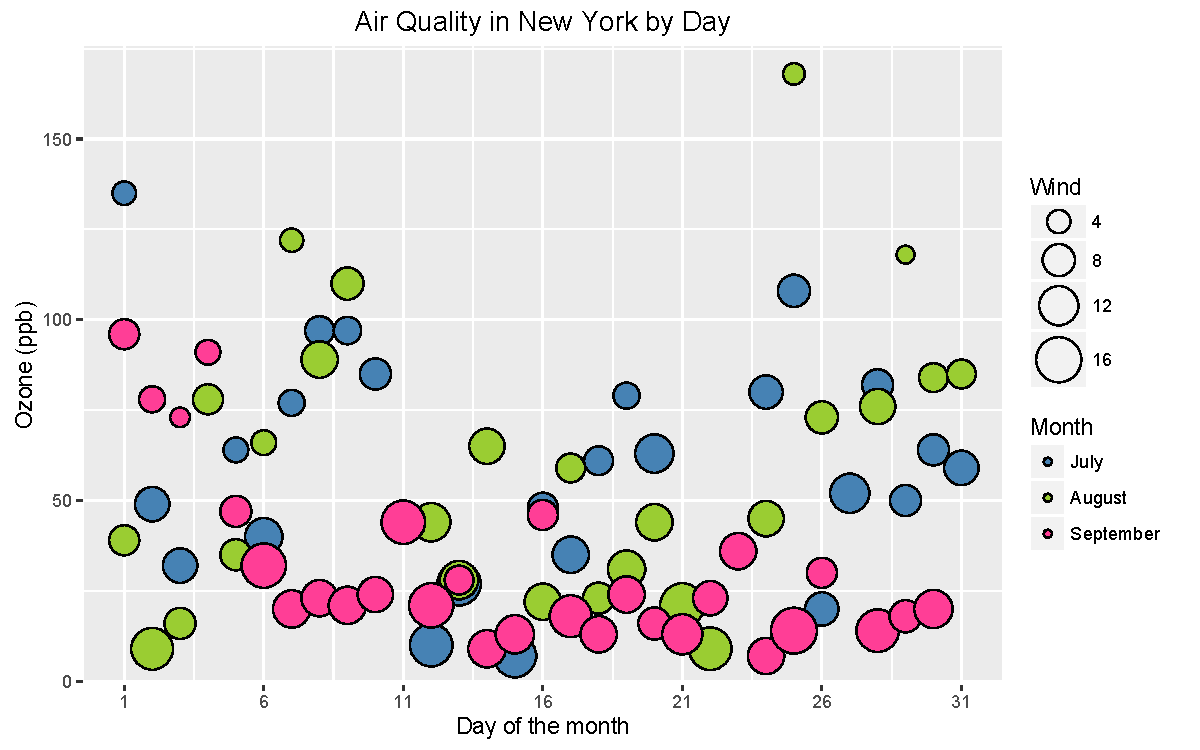
\includegraphics[width=0.6\linewidth]{6_Weighted_Scatterplots_pdf/wscatter_12-1} \end{center}

For our graph, this makes the pattern for \texttt{Wind} a little hard to
see. Another way to adjust the size of the data points is to use
\texttt{scale\_size} and specify a desired range.

\begin{Shaded}
\begin{Highlighting}[]
\NormalTok{p6 <-}\StringTok{ }\KeywordTok{ggplot}\NormalTok{(aq_trim, }\KeywordTok{aes}\NormalTok{(}\DataTypeTok{x =} \NormalTok{Day, }\DataTypeTok{y =} \NormalTok{Ozone, }\DataTypeTok{size =} \NormalTok{Wind, }\DataTypeTok{fill =} \NormalTok{Month)) +}\StringTok{ }
\StringTok{  }\KeywordTok{geom_point}\NormalTok{(}\DataTypeTok{shape =} \DecValTok{21}\NormalTok{) +}
\StringTok{  }\KeywordTok{ggtitle}\NormalTok{(}\StringTok{"Air Quality in New York by Day"}\NormalTok{) +}\StringTok{ }
\StringTok{  }\KeywordTok{labs}\NormalTok{(}\DataTypeTok{x =} \StringTok{"Day of the month"}\NormalTok{, }\DataTypeTok{y =} \StringTok{"Ozone (ppb)"}\NormalTok{) +}
\StringTok{  }\KeywordTok{scale_x_continuous}\NormalTok{(}\DataTypeTok{breaks =} \KeywordTok{seq}\NormalTok{(}\DecValTok{1}\NormalTok{, }\DecValTok{31}\NormalTok{, }\DecValTok{5}\NormalTok{)) +}
\StringTok{  }\KeywordTok{scale_fill_manual}\NormalTok{(}\DataTypeTok{values =} \NormalTok{fill) +}
\StringTok{  }\KeywordTok{scale_size}\NormalTok{(}\DataTypeTok{range =} \KeywordTok{c}\NormalTok{(}\DecValTok{1}\NormalTok{, }\DecValTok{10}\NormalTok{))}
\NormalTok{p6}
\end{Highlighting}
\end{Shaded}

\begin{center}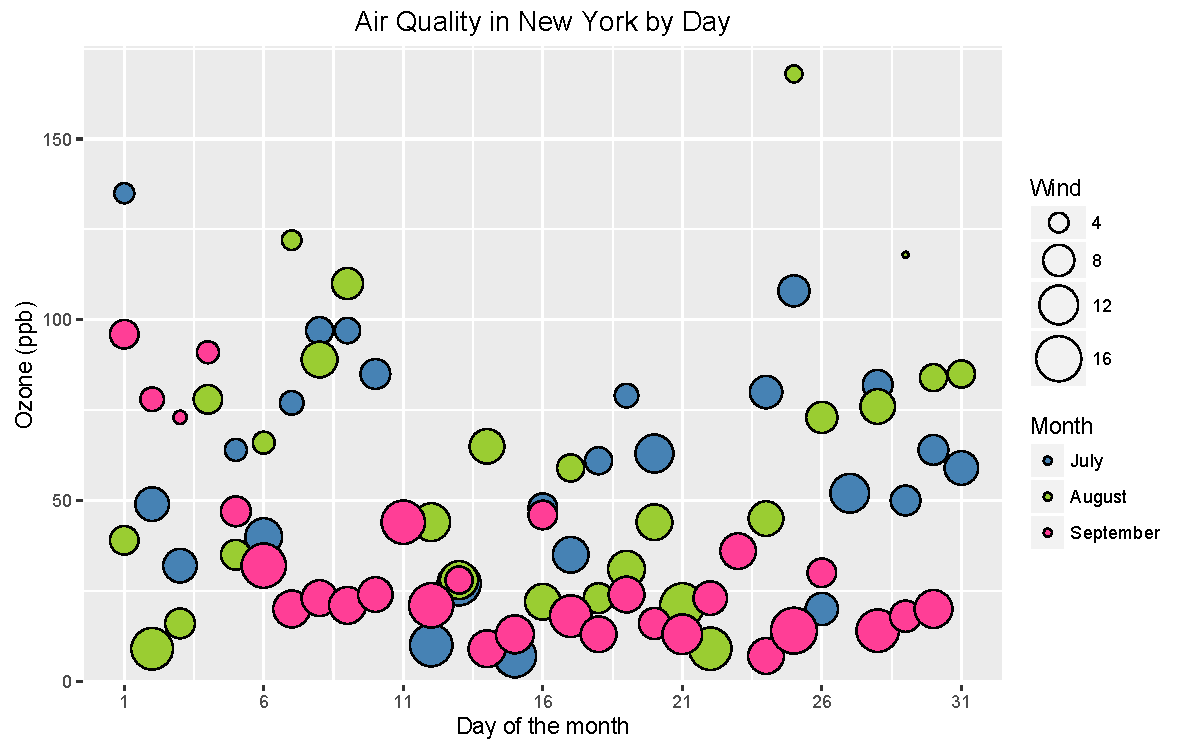
\includegraphics[width=0.6\linewidth]{6_Weighted_Scatterplots_pdf/wscatter_13-1} \end{center}

\section{Adjusting legend position}\label{adjusting-legend-position}

To adjust the position of the legend from the default spot of right of
the graph, we add the \texttt{theme} option and specify the
\texttt{legend.position\ =\ "bottom"} argument. We can also change the
legend shape using the \texttt{legend.direction\ =\ "horizontal"}
argument.

\begin{Shaded}
\begin{Highlighting}[]
\NormalTok{p6 <-}\StringTok{ }\NormalTok{p6 +}\StringTok{ }\KeywordTok{theme}\NormalTok{(}\DataTypeTok{legend.position =} \StringTok{"bottom"}\NormalTok{, }\DataTypeTok{legend.direction =} \StringTok{"horizontal"}\NormalTok{)}
\NormalTok{p6}
\end{Highlighting}
\end{Shaded}

\begin{center}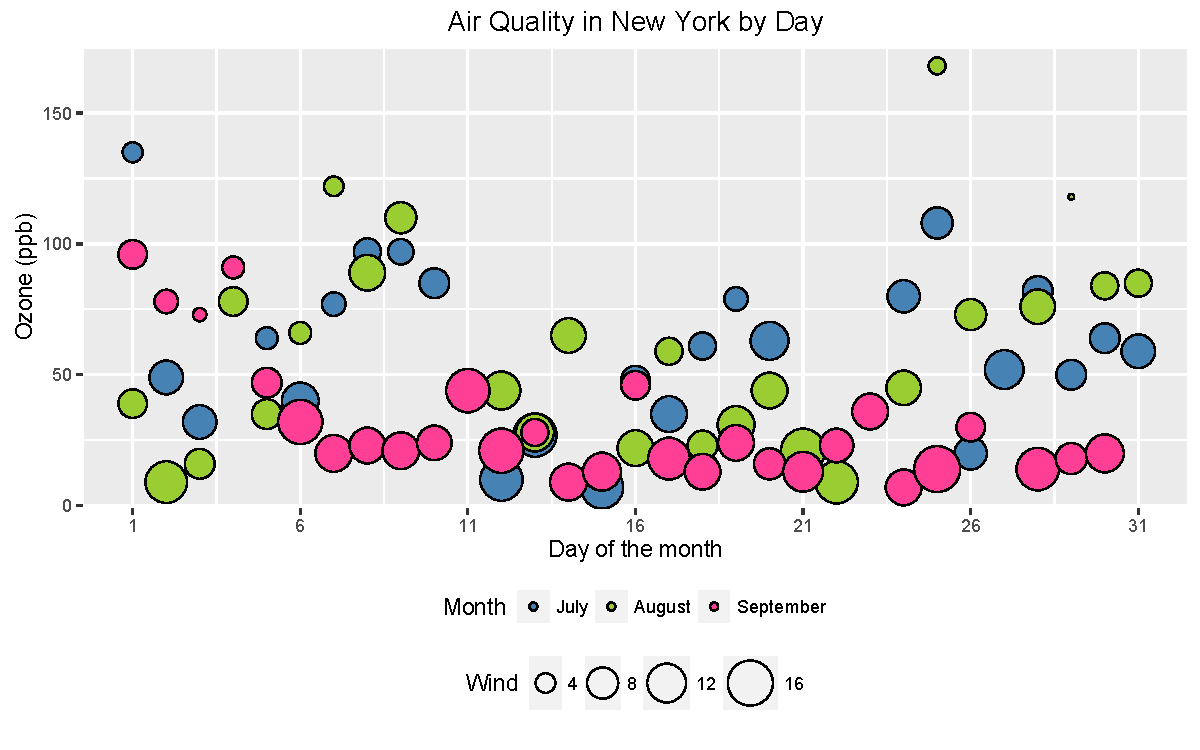
\includegraphics[width=0.6\linewidth]{6_Weighted_Scatterplots_pdf/wscatter_14-1} \end{center}

\section{Changing the legend titles}\label{changing-the-legend-titles}

To change the titles of the two legends, we use the \texttt{labs}
option. In order to tell ggplot2 exactly what legend you're referring
to, just have a look in the \texttt{ggplot} option and see what argument
you used to create the legend in the first place. In this case we used
the \texttt{size} argument for ``Wind'' and \texttt{fill} for ``Month'',
so we pass these to \texttt{labs} with our new titles.

\begin{Shaded}
\begin{Highlighting}[]
\NormalTok{p6 <-}\StringTok{ }\NormalTok{p6 +}\StringTok{ }\KeywordTok{labs}\NormalTok{(}\DataTypeTok{size =} \StringTok{"Wind Speed (mph) "}\NormalTok{, }\DataTypeTok{fill =} \StringTok{"Months "}\NormalTok{)}
\NormalTok{p6}
\end{Highlighting}
\end{Shaded}

\begin{center}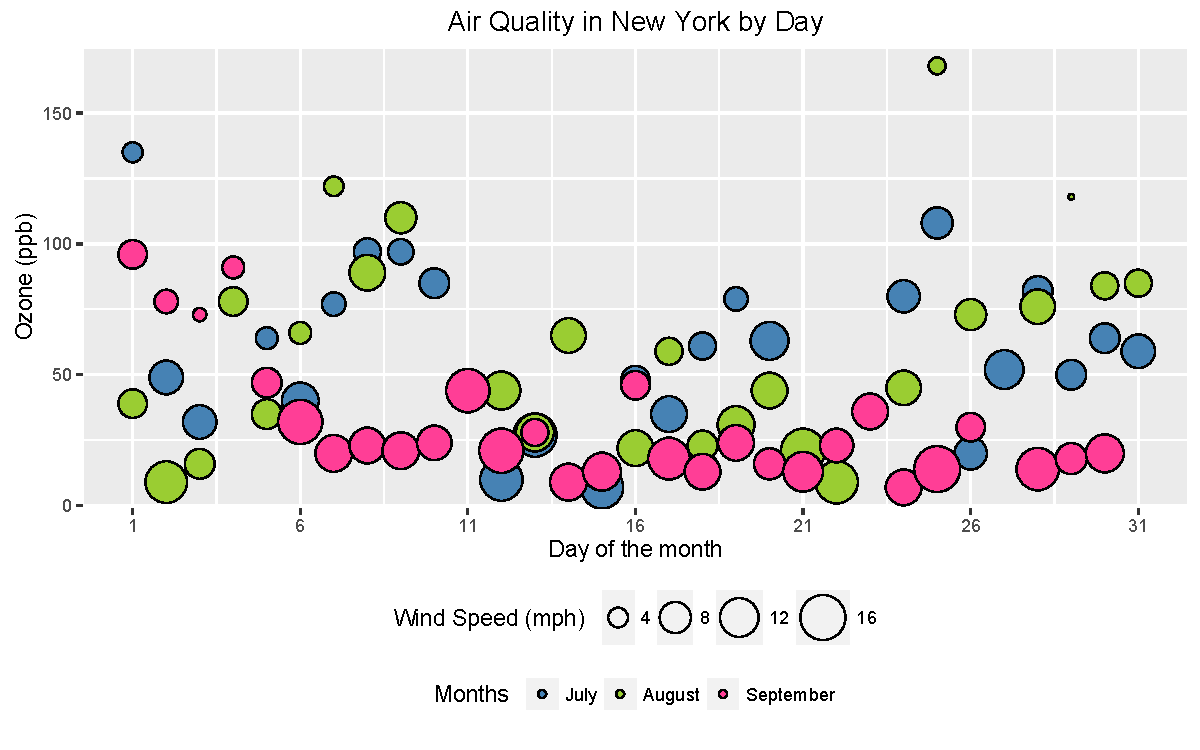
\includegraphics[width=0.6\linewidth]{6_Weighted_Scatterplots_pdf/wscatter_15-1} \end{center}

\section{Creating horizontal legends}\label{creating-horizontal-legends}

It looks a little awkward having the two titles sitting on top of each
other, as well as taking up unnecessary space. To place the legends next
to each other, we use the \texttt{legend.box\ =\ "horizontal"} argument
in \texttt{theme}. Because the boxes around the legend keys aren't even
in each of the legends, this means the legends don't align properly. To
fix this, we change the box size around the legend keys using
\texttt{legend.key.size}. We need to load in the \texttt{grid} package
to get this argument to work.

\begin{Shaded}
\begin{Highlighting}[]
\NormalTok{p6 <-}\StringTok{ }\NormalTok{p6 +}\StringTok{ }\KeywordTok{theme}\NormalTok{(}\DataTypeTok{legend.box =} \StringTok{"horizontal"}\NormalTok{, }\DataTypeTok{legend.key.size =} \KeywordTok{unit}\NormalTok{(}\DecValTok{1}\NormalTok{, }\StringTok{"cm"}\NormalTok{))}
\NormalTok{p6}
\end{Highlighting}
\end{Shaded}

\begin{center}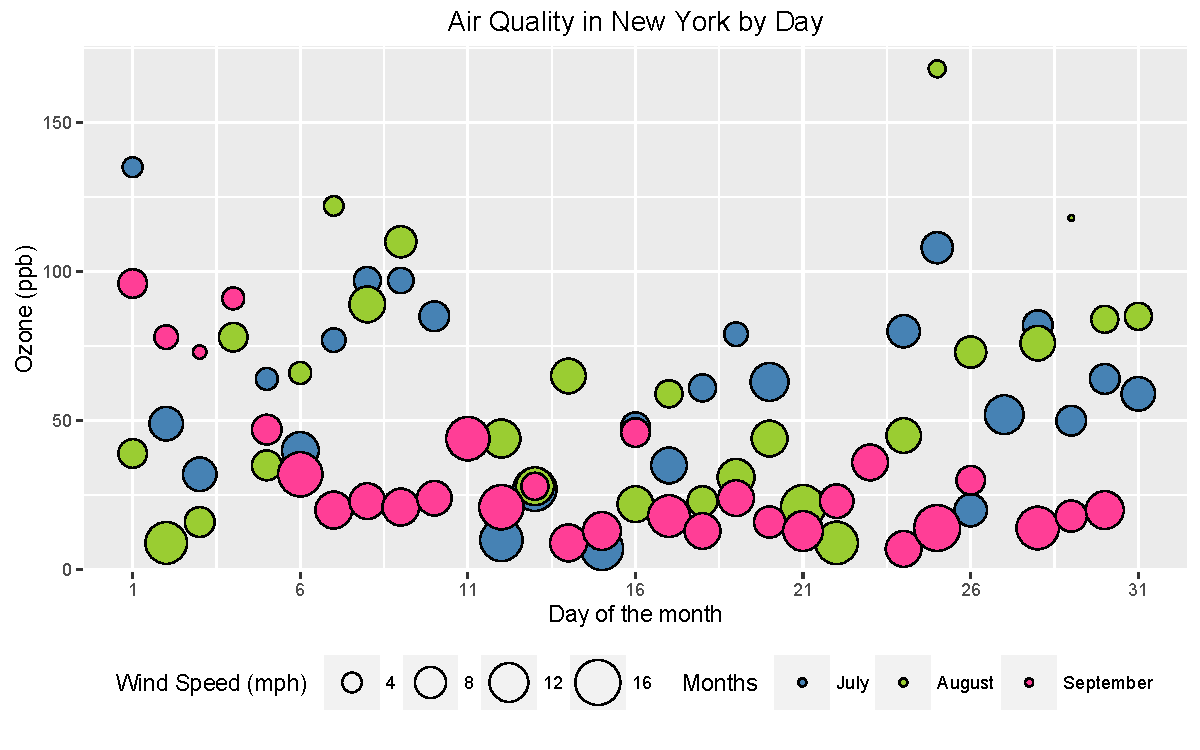
\includegraphics[width=0.6\linewidth]{6_Weighted_Scatterplots_pdf/wscatter_16-1} \end{center}

\section{Using the white theme}\label{using-the-white-theme}

As explained in the previous posts, we can also change the overall look
of the plot using themes. We'll start using a simple theme customisation
by adding \texttt{theme\_bw()} after \texttt{ggplot()}. As you can see,
we can further tweak the graph using the \texttt{theme} option, which
we've used so far to change the legend.

\begin{Shaded}
\begin{Highlighting}[]
\NormalTok{p6 <-}\StringTok{ }\KeywordTok{ggplot}\NormalTok{(aq_trim, }\KeywordTok{aes}\NormalTok{(}\DataTypeTok{x =} \NormalTok{Day, }\DataTypeTok{y =} \NormalTok{Ozone, }\DataTypeTok{size =} \NormalTok{Wind, }\DataTypeTok{fill =} \NormalTok{Month)) +}
\StringTok{  }\KeywordTok{geom_point}\NormalTok{(}\DataTypeTok{shape =} \DecValTok{21}\NormalTok{) +}
\StringTok{  }\KeywordTok{ggtitle}\NormalTok{(}\StringTok{"Air Quality in New York by Day"}\NormalTok{) +}\StringTok{ }
\StringTok{  }\KeywordTok{labs}\NormalTok{(}\DataTypeTok{x =} \StringTok{"Day of the month"}\NormalTok{, }\DataTypeTok{y =} \StringTok{"Ozone (ppb)"}\NormalTok{,}
    \DataTypeTok{size =} \StringTok{"Wind Speed (mph) "}\NormalTok{, }\DataTypeTok{fill =} \StringTok{"Months "}\NormalTok{) +}
\StringTok{  }\KeywordTok{scale_x_continuous}\NormalTok{(}\DataTypeTok{breaks =} \KeywordTok{seq}\NormalTok{(}\DecValTok{1}\NormalTok{, }\DecValTok{31}\NormalTok{, }\DecValTok{5}\NormalTok{)) +}
\StringTok{  }\KeywordTok{scale_fill_manual}\NormalTok{(}\DataTypeTok{values =} \NormalTok{fill) +}
\StringTok{  }\KeywordTok{scale_size}\NormalTok{(}\DataTypeTok{range =} \KeywordTok{c}\NormalTok{(}\DecValTok{1}\NormalTok{, }\DecValTok{10}\NormalTok{)) +}
\StringTok{  }\KeywordTok{theme_bw}\NormalTok{() +}
\StringTok{  }\KeywordTok{theme}\NormalTok{(}\DataTypeTok{legend.position=}\StringTok{"bottom"}\NormalTok{, }\DataTypeTok{legend.direction=}\StringTok{"horizontal"}\NormalTok{,}
    \DataTypeTok{legend.box =} \StringTok{"horizontal"}\NormalTok{, }
    \DataTypeTok{legend.key.size =} \KeywordTok{unit}\NormalTok{(}\DecValTok{1}\NormalTok{, }\StringTok{"cm"}\NormalTok{))}
\NormalTok{p6}
\end{Highlighting}
\end{Shaded}

\begin{center}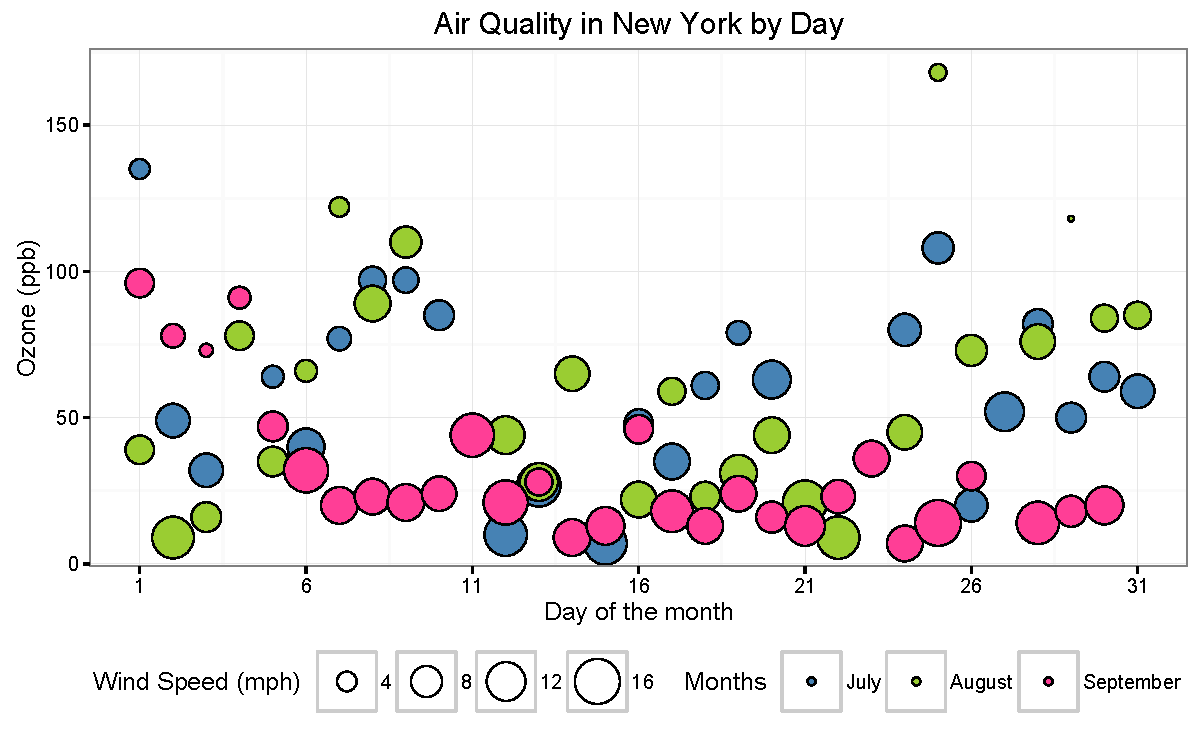
\includegraphics[width=0.6\linewidth]{6_Weighted_Scatterplots_pdf/wscatter_17-1} \end{center}

\section{Creating an XKCD style
chart}\label{creating-an-xkcd-style-chart}

Of course, you may want to create your own themes as well.
\texttt{ggplot2} allows for a very high degree of customisation,
including allowing you to use imported fonts. Below is an example of a
theme Mauricio was able to create which mimics the visual style of
\href{http://xkcd.com/}{XKCD}. In order to create this chart, you first
need to import the XKCD font, and load it into R using the
\texttt{extrafont} package.

\begin{Shaded}
\begin{Highlighting}[]
\NormalTok{fill <-}\StringTok{ }\KeywordTok{c}\NormalTok{(}\StringTok{"#56B4E9"}\NormalTok{, }\StringTok{"#F0E442"}\NormalTok{, }\StringTok{"violetred1"}\NormalTok{)}

\NormalTok{p6 <-}\StringTok{ }\KeywordTok{ggplot}\NormalTok{(aq_trim, }\KeywordTok{aes}\NormalTok{(}\DataTypeTok{x =} \NormalTok{Day, }\DataTypeTok{y =} \NormalTok{Ozone, }\DataTypeTok{size =} \NormalTok{Wind, }\DataTypeTok{fill =} \NormalTok{Month)) +}\StringTok{ }
\StringTok{  }\KeywordTok{geom_point}\NormalTok{(}\DataTypeTok{shape =} \DecValTok{21}\NormalTok{) +}
\StringTok{  }\KeywordTok{ggtitle}\NormalTok{(}\StringTok{"Air Quality in New York by Day"}\NormalTok{) +}\StringTok{ }
\StringTok{  }\KeywordTok{labs}\NormalTok{(}\DataTypeTok{x =} \StringTok{"Day of the month"}\NormalTok{, }\DataTypeTok{y =} \StringTok{"Ozone (ppb)"}\NormalTok{,}
    \DataTypeTok{size =} \StringTok{"Wind Speed (mph) "}\NormalTok{, }\DataTypeTok{fill =} \StringTok{"Months "}\NormalTok{) +}
\StringTok{  }\KeywordTok{scale_x_continuous}\NormalTok{(}\DataTypeTok{breaks =} \KeywordTok{seq}\NormalTok{(}\DecValTok{1}\NormalTok{, }\DecValTok{31}\NormalTok{, }\DecValTok{5}\NormalTok{)) +}
\StringTok{  }\KeywordTok{scale_fill_manual}\NormalTok{(}\DataTypeTok{values =} \NormalTok{fill) +}
\StringTok{  }\KeywordTok{scale_size}\NormalTok{(}\DataTypeTok{range =} \KeywordTok{c}\NormalTok{(}\DecValTok{1}\NormalTok{, }\DecValTok{10}\NormalTok{)) +}
\StringTok{  }\KeywordTok{theme}\NormalTok{(}\DataTypeTok{axis.line.x =} \KeywordTok{element_line}\NormalTok{(}\DataTypeTok{size=}\NormalTok{.}\DecValTok{5}\NormalTok{, }\DataTypeTok{colour =} \StringTok{"black"}\NormalTok{), }
    \DataTypeTok{axis.line.y =} \KeywordTok{element_line}\NormalTok{(}\DataTypeTok{size=}\NormalTok{.}\DecValTok{5}\NormalTok{, }\DataTypeTok{colour =} \StringTok{"black"}\NormalTok{),     }
    \DataTypeTok{axis.text.x=}\KeywordTok{element_text}\NormalTok{(}\DataTypeTok{colour=}\StringTok{"black"}\NormalTok{, }\DataTypeTok{size =} \DecValTok{10}\NormalTok{), }
    \DataTypeTok{axis.text.y=}\KeywordTok{element_text}\NormalTok{(}\DataTypeTok{colour=}\StringTok{"black"}\NormalTok{, }\DataTypeTok{size =} \DecValTok{10}\NormalTok{), }
    \DataTypeTok{legend.position=}\StringTok{"bottom"}\NormalTok{, }
    \DataTypeTok{legend.direction=}\StringTok{"horizontal"}\NormalTok{,}
    \DataTypeTok{legend.box =} \StringTok{"horizontal"}\NormalTok{, }
    \DataTypeTok{legend.key.size =} \KeywordTok{unit}\NormalTok{(}\DecValTok{1}\NormalTok{, }\StringTok{"cm"}\NormalTok{),}
    \DataTypeTok{legend.key =} \KeywordTok{element_blank}\NormalTok{(),}
    \DataTypeTok{panel.grid.major =} \KeywordTok{element_blank}\NormalTok{(),}
    \DataTypeTok{panel.grid.minor =} \KeywordTok{element_blank}\NormalTok{(), }
    \DataTypeTok{panel.border =} \KeywordTok{element_blank}\NormalTok{(),}
    \DataTypeTok{panel.background =} \KeywordTok{element_blank}\NormalTok{(),}
    \DataTypeTok{plot.title=}\KeywordTok{element_text}\NormalTok{(}\DataTypeTok{family=}\StringTok{"xkcd-Regular"}\NormalTok{), }
    \DataTypeTok{text=}\KeywordTok{element_text}\NormalTok{(}\DataTypeTok{family=}\StringTok{"xkcd-Regular"}\NormalTok{)) }
\NormalTok{p6}
\end{Highlighting}
\end{Shaded}

\begin{center}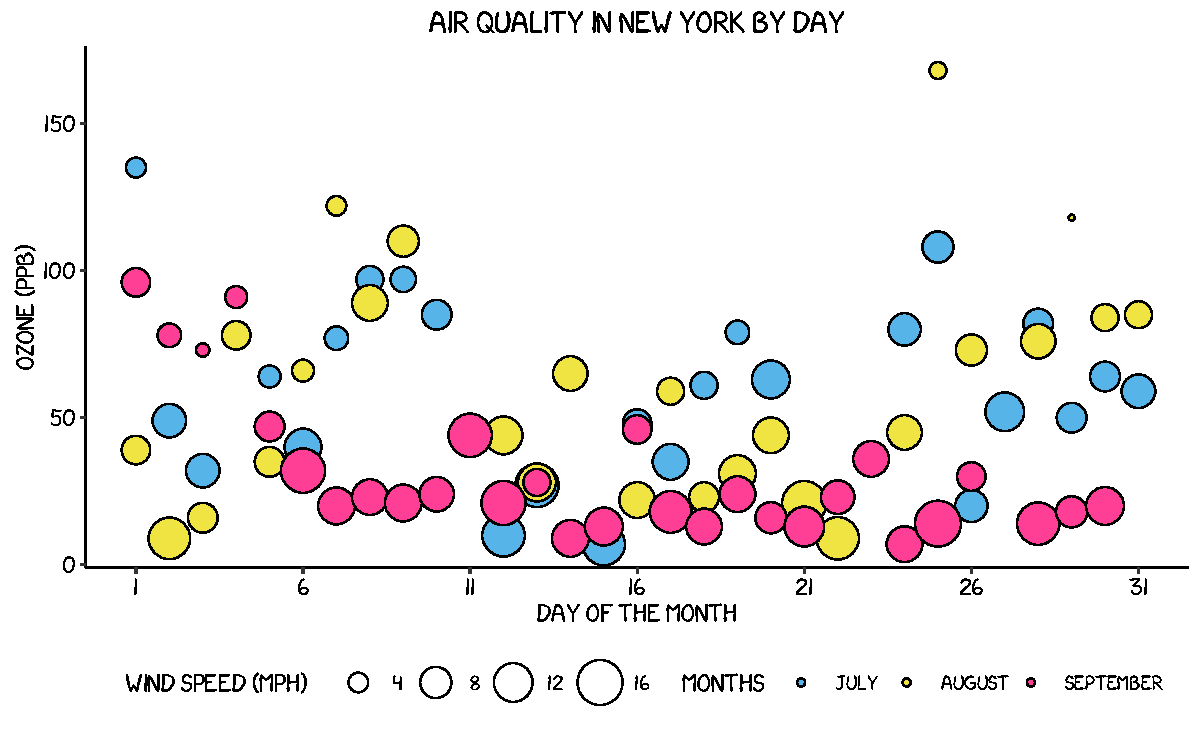
\includegraphics[width=0.6\linewidth]{6_Weighted_Scatterplots_pdf/wscatter_18-1} \end{center}

\section{\texorpdfstring{Using `The Economist'
theme}{Using The Economist theme}}\label{using-the-economist-theme}

There are a wider range of pre-built themes available as part of the
\texttt{ggthemes} package (more information on these
\href{https://cran.r-project.org/web/packages/ggthemes/vignettes/ggthemes.html}{here}).
Below we've applied \texttt{theme\_economist()}, which approximates
graphs in the Economist magazine. It is also important that the font
change argument inside \texttt{theme} is optional and it's only to
obtain a more similar result compared to the original. For an exact
result you need `Officina Sans' which is a commercial font and is
available \href{http://www.myfonts.com/fonts/itc/officina-sans/}{here}.

\begin{Shaded}
\begin{Highlighting}[]
\NormalTok{p6 <-}\StringTok{ }\KeywordTok{ggplot}\NormalTok{(aq_trim, }\KeywordTok{aes}\NormalTok{(}\DataTypeTok{x =} \NormalTok{Day, }\DataTypeTok{y =} \NormalTok{Ozone, }\DataTypeTok{size =} \NormalTok{Wind, }\DataTypeTok{fill =} \NormalTok{Month)) +}
\StringTok{  }\KeywordTok{geom_point}\NormalTok{(}\DataTypeTok{shape =} \DecValTok{21}\NormalTok{) +}
\StringTok{  }\KeywordTok{ggtitle}\NormalTok{(}\StringTok{"Air Quality in New York by Day"}\NormalTok{) +}\StringTok{ }
\StringTok{  }\KeywordTok{labs}\NormalTok{(}\DataTypeTok{x =} \StringTok{"Day of the month"}\NormalTok{, }\DataTypeTok{y =} \StringTok{"Ozone (ppb)"}\NormalTok{, }\DataTypeTok{size =} \StringTok{"Wind Speed (mph) "}\NormalTok{, }
    \DataTypeTok{fill =} \StringTok{"Months "}\NormalTok{) +}
\StringTok{  }\KeywordTok{scale_x_continuous}\NormalTok{(}\DataTypeTok{breaks =} \KeywordTok{seq}\NormalTok{(}\DecValTok{1}\NormalTok{, }\DecValTok{31}\NormalTok{, }\DecValTok{5}\NormalTok{)) +}
\StringTok{  }\KeywordTok{scale_size}\NormalTok{(}\DataTypeTok{range =} \KeywordTok{c}\NormalTok{(}\DecValTok{1}\NormalTok{, }\DecValTok{10}\NormalTok{)) +}
\StringTok{  }\KeywordTok{theme_economist}\NormalTok{() +}\StringTok{ }\KeywordTok{scale_fill_economist}\NormalTok{() +}
\StringTok{  }\KeywordTok{theme}\NormalTok{(}\DataTypeTok{axis.line.x =} \KeywordTok{element_line}\NormalTok{(}\DataTypeTok{size=}\NormalTok{.}\DecValTok{5}\NormalTok{, }\DataTypeTok{colour =} \StringTok{"black"}\NormalTok{),}
    \DataTypeTok{axis.title =} \KeywordTok{element_text}\NormalTok{(}\DataTypeTok{size =} \DecValTok{12}\NormalTok{),}
    \DataTypeTok{legend.position=}\StringTok{"bottom"}\NormalTok{, }
    \DataTypeTok{legend.direction=}\StringTok{"horizontal"}\NormalTok{,}
    \DataTypeTok{legend.box =} \StringTok{"horizontal"}\NormalTok{, }
    \DataTypeTok{legend.key.size =} \KeywordTok{unit}\NormalTok{(}\DecValTok{1}\NormalTok{, }\StringTok{"cm"}\NormalTok{),}
    \DataTypeTok{legend.text =} \KeywordTok{element_text}\NormalTok{(}\DataTypeTok{size =} \DecValTok{10}\NormalTok{),}
    \DataTypeTok{text =} \KeywordTok{element_text}\NormalTok{(}\DataTypeTok{family =} \StringTok{"OfficinaSanITC-Book"}\NormalTok{),}
    \DataTypeTok{plot.title =} \KeywordTok{element_text}\NormalTok{(}\DataTypeTok{family=}\StringTok{"OfficinaSanITC-Book"}\NormalTok{))}
\NormalTok{p6}
\end{Highlighting}
\end{Shaded}

\begin{center}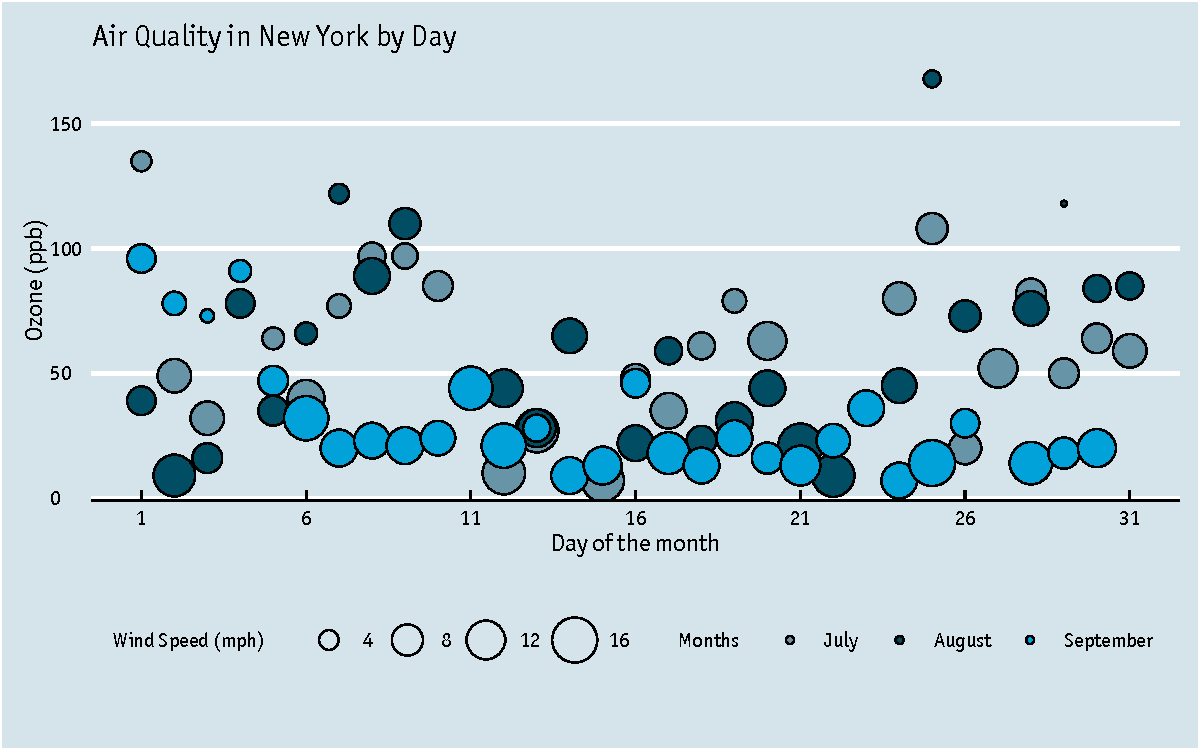
\includegraphics[width=0.6\linewidth]{6_Weighted_Scatterplots_pdf/wscatter_19-1} \end{center}

\section{\texorpdfstring{Using `Five Thirty Eight'
theme}{Using Five Thirty Eight theme}}\label{using-five-thirty-eight-theme}

Below we've applied \texttt{theme\_fivethirtyeight()}, which
approximates graphs in the nice
\href{http://fivethirtyeight.com/}{FiveThirtyEight} website. Again, it
is also important that the font change is optional and it's only to
obtain a more similar result compared to the original. For an exact
result you need `Atlas Grotesk' and `Decima Mono Pro' which are
commercial font and are available
\href{https://commercialtype.com/catalog/atlas}{here} and
\href{https://www.myfonts.com/fonts/tipografiaramis/decima-mono-pro/}{here}.

\begin{Shaded}
\begin{Highlighting}[]
\NormalTok{p6 <-}\StringTok{ }\KeywordTok{ggplot}\NormalTok{(aq_trim, }\KeywordTok{aes}\NormalTok{(}\DataTypeTok{x =} \NormalTok{Day, }\DataTypeTok{y =} \NormalTok{Ozone, }\DataTypeTok{size =} \NormalTok{Wind, }\DataTypeTok{fill =} \NormalTok{Month)) +}
\StringTok{  }\KeywordTok{geom_point}\NormalTok{(}\DataTypeTok{shape =} \DecValTok{21}\NormalTok{) +}
\StringTok{  }\KeywordTok{ggtitle}\NormalTok{(}\StringTok{"Air Quality in New York by Day"}\NormalTok{) +}\StringTok{ }
\StringTok{  }\KeywordTok{labs}\NormalTok{(}\DataTypeTok{x =} \StringTok{"Day of the month"}\NormalTok{, }\DataTypeTok{y =} \StringTok{"Ozone (ppb)"}\NormalTok{, }\DataTypeTok{size =} \StringTok{"Wind Speed (mph) "}\NormalTok{, }
    \DataTypeTok{fill =} \StringTok{"Months "}\NormalTok{) +}
\StringTok{  }\KeywordTok{scale_x_continuous}\NormalTok{(}\DataTypeTok{breaks =} \KeywordTok{seq}\NormalTok{(}\DecValTok{1}\NormalTok{, }\DecValTok{31}\NormalTok{, }\DecValTok{5}\NormalTok{)) +}
\StringTok{  }\KeywordTok{scale_size}\NormalTok{(}\DataTypeTok{range =} \KeywordTok{c}\NormalTok{(}\DecValTok{1}\NormalTok{, }\DecValTok{10}\NormalTok{)) +}
\StringTok{  }\KeywordTok{theme_fivethirtyeight}\NormalTok{() +}\StringTok{ }\KeywordTok{scale_fill_fivethirtyeight}\NormalTok{() +}\StringTok{   }
\StringTok{  }\KeywordTok{theme}\NormalTok{(}\DataTypeTok{axis.title =} \KeywordTok{element_text}\NormalTok{(}\DataTypeTok{family=}\StringTok{"Atlas Grotesk Regular"}\NormalTok{),}
    \DataTypeTok{legend.position=}\StringTok{"bottom"}\NormalTok{, }
    \DataTypeTok{legend.direction=}\StringTok{"horizontal"}\NormalTok{,}
    \DataTypeTok{legend.box =} \StringTok{"horizontal"}\NormalTok{, }
    \DataTypeTok{legend.key.size =} \KeywordTok{unit}\NormalTok{(}\DecValTok{1}\NormalTok{, }\StringTok{"cm"}\NormalTok{),}
    \DataTypeTok{legend.title=}\KeywordTok{element_text}\NormalTok{(}\DataTypeTok{family=}\StringTok{"Atlas Grotesk Regular"}\NormalTok{, }\DataTypeTok{size =} \DecValTok{10}\NormalTok{),}
    \DataTypeTok{legend.text=}\KeywordTok{element_text}\NormalTok{(}\DataTypeTok{family=}\StringTok{"Atlas Grotesk Regular"}\NormalTok{, }\DataTypeTok{size =} \DecValTok{10}\NormalTok{),}
    \DataTypeTok{plot.title=}\KeywordTok{element_text}\NormalTok{(}\DataTypeTok{family=}\StringTok{"Atlas Grotesk Medium"}\NormalTok{), }
    \DataTypeTok{text=}\KeywordTok{element_text}\NormalTok{(}\DataTypeTok{family=}\StringTok{"DecimaMonoPro"}\NormalTok{)) }
\NormalTok{p6}
\end{Highlighting}
\end{Shaded}

\begin{center}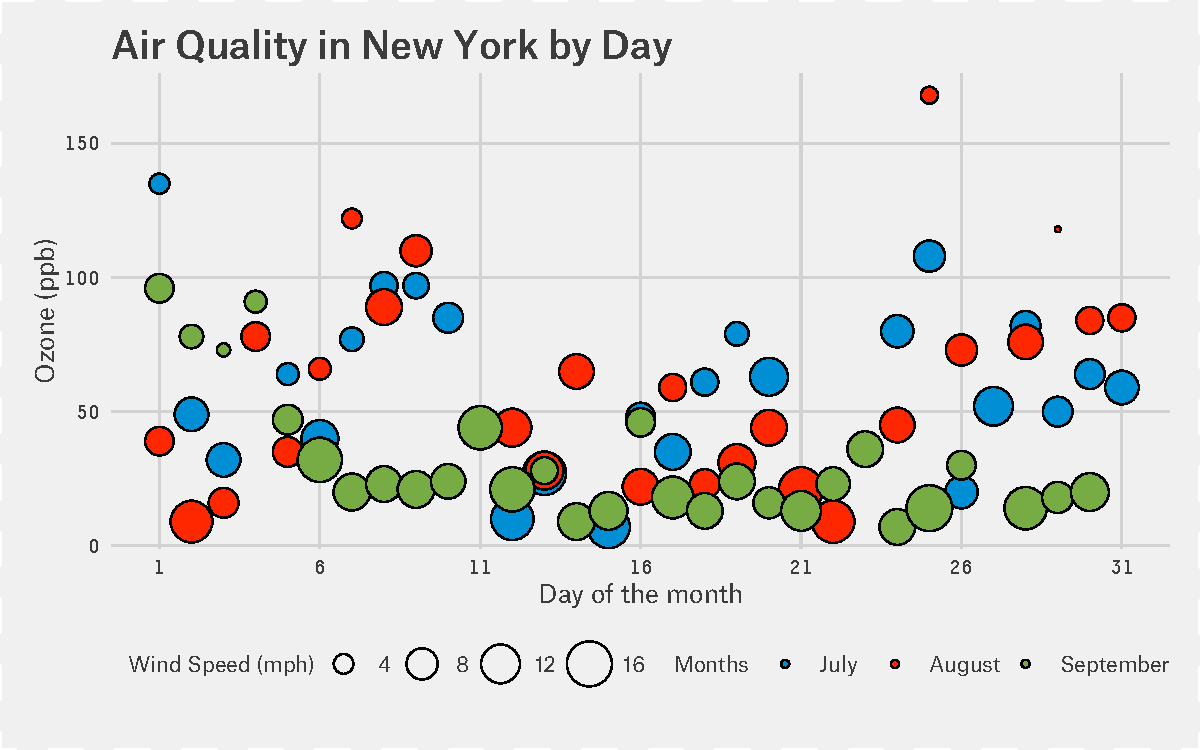
\includegraphics[width=0.6\linewidth]{6_Weighted_Scatterplots_pdf/wscatter_20-1} \end{center}

\section{Creating your own theme}\label{creating-your-own-theme}

As before, you can modify your plots a lot as \texttt{ggplot2} allows
many customisations. Here we present our original result shown at the
top of page.

\begin{Shaded}
\begin{Highlighting}[]
\NormalTok{fill =}\StringTok{ }\KeywordTok{c}\NormalTok{(}\StringTok{"steelblue"}\NormalTok{, }\StringTok{"yellowgreen"}\NormalTok{, }\StringTok{"violetred1"}\NormalTok{)}

\NormalTok{p6 <-}\StringTok{ }\KeywordTok{ggplot}\NormalTok{(aq_trim, }\KeywordTok{aes}\NormalTok{(}\DataTypeTok{x =} \NormalTok{Day, }\DataTypeTok{y =} \NormalTok{Ozone, }\DataTypeTok{size =} \NormalTok{Wind, }\DataTypeTok{fill =} \NormalTok{Month)) +}
\StringTok{  }\KeywordTok{geom_point}\NormalTok{(}\DataTypeTok{shape =} \DecValTok{21}\NormalTok{) +}
\StringTok{  }\KeywordTok{ggtitle}\NormalTok{(}\StringTok{"Air Quality in New York by Day"}\NormalTok{) +}\StringTok{ }
\StringTok{  }\KeywordTok{labs}\NormalTok{(}\DataTypeTok{x =} \StringTok{"Day of the month"}\NormalTok{, }\DataTypeTok{y =} \StringTok{"Ozone (ppb)"}\NormalTok{, }\DataTypeTok{size =} \StringTok{"Wind Speed (mph) "}\NormalTok{, }
    \DataTypeTok{fill =} \StringTok{"Months "}\NormalTok{) +}
\StringTok{  }\KeywordTok{scale_x_continuous}\NormalTok{(}\DataTypeTok{breaks =} \KeywordTok{seq}\NormalTok{(}\DecValTok{1}\NormalTok{, }\DecValTok{31}\NormalTok{, }\DecValTok{5}\NormalTok{)) +}
\StringTok{  }\KeywordTok{scale_size}\NormalTok{(}\DataTypeTok{range =} \KeywordTok{c}\NormalTok{(}\DecValTok{1}\NormalTok{, }\DecValTok{10}\NormalTok{)) +}
\StringTok{  }\KeywordTok{scale_fill_manual}\NormalTok{(}\DataTypeTok{values =} \NormalTok{fill) +}
\StringTok{  }\KeywordTok{theme}\NormalTok{(}\DataTypeTok{panel.border =} \KeywordTok{element_rect}\NormalTok{(}\DataTypeTok{colour =} \StringTok{"black"}\NormalTok{, }\DataTypeTok{fill=}\OtherTok{NA}\NormalTok{, }\DataTypeTok{size=}\NormalTok{.}\DecValTok{5}\NormalTok{), }
    \DataTypeTok{axis.text.x=}\KeywordTok{element_text}\NormalTok{(}\DataTypeTok{colour=}\StringTok{"black"}\NormalTok{, }\DataTypeTok{size =} \DecValTok{9}\NormalTok{), }
    \DataTypeTok{axis.text.y=}\KeywordTok{element_text}\NormalTok{(}\DataTypeTok{colour=}\StringTok{"black"}\NormalTok{, }\DataTypeTok{size =} \DecValTok{9}\NormalTok{),}
    \DataTypeTok{legend.position=}\StringTok{"bottom"}\NormalTok{, }
    \DataTypeTok{legend.direction=}\StringTok{"horizontal"}\NormalTok{,}
    \DataTypeTok{legend.box =} \StringTok{"horizontal"}\NormalTok{, }
    \DataTypeTok{legend.key.size =} \KeywordTok{unit}\NormalTok{(}\DecValTok{1}\NormalTok{, }\StringTok{"cm"}\NormalTok{),}
    \DataTypeTok{legend.key =} \KeywordTok{element_blank}\NormalTok{(),}
    \DataTypeTok{panel.grid.major =} \KeywordTok{element_line}\NormalTok{(}\DataTypeTok{colour =} \StringTok{"#d3d3d3"}\NormalTok{), }
    \DataTypeTok{panel.grid.minor =} \KeywordTok{element_blank}\NormalTok{(), }
    \DataTypeTok{panel.border =} \KeywordTok{element_blank}\NormalTok{(), }\DataTypeTok{panel.background =} \KeywordTok{element_blank}\NormalTok{(),}
    \DataTypeTok{plot.title =} \KeywordTok{element_text}\NormalTok{(}\DataTypeTok{size =} \DecValTok{14}\NormalTok{, }\DataTypeTok{family =} \StringTok{"Tahoma"}\NormalTok{, }\DataTypeTok{face =} \StringTok{"bold"}\NormalTok{),}
    \DataTypeTok{text=}\KeywordTok{element_text}\NormalTok{(}\DataTypeTok{family=}\StringTok{"Tahoma"}\NormalTok{)) }
\NormalTok{p6}
\end{Highlighting}
\end{Shaded}

\begin{center}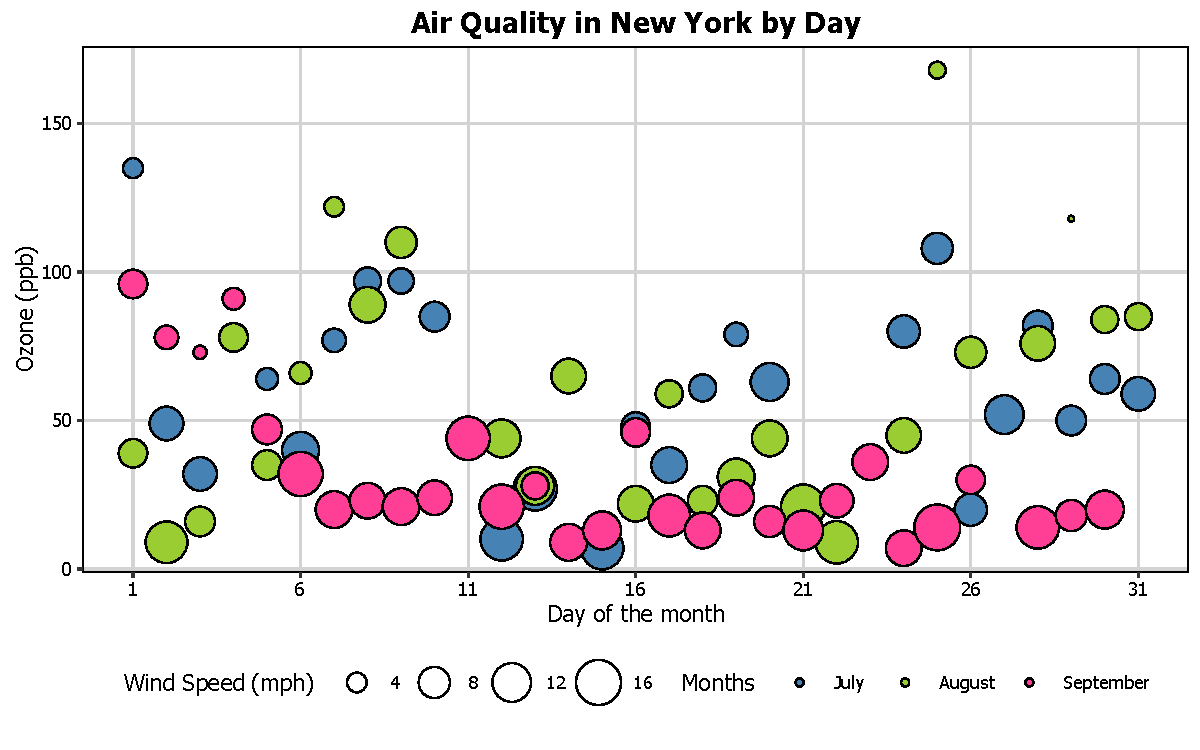
\includegraphics[width=0.6\linewidth]{6_Weighted_Scatterplots_pdf/wscatter_21-1} \end{center}
